\chapter{Experiments}\label{ch:experiments}
In this chapter we present experiments held to evaluate how the pruning with
heuristic affects MobileNet v1\cite{howard2017mobilenets} based models. The
experiments have been run using both CIFAR-10\cite{cifar_10} and ImageNet
2012\cite{imagenet_cvpr09}.
An overview of MobileNet v1 architecture and a presentation the datasets used
in the experiments is given, while experimental results are finally reported.

\section{MobileNet v1}
MobileNet is a class of efficient models for mobile and embedded vision
applications (\autoref{fig:mobilenet_applications}) developed by Google.
It is based on a streamlined architecture that uses depthwise separable
convolutions to build light weight deep neural networks.

\begin{figure}[ht]
    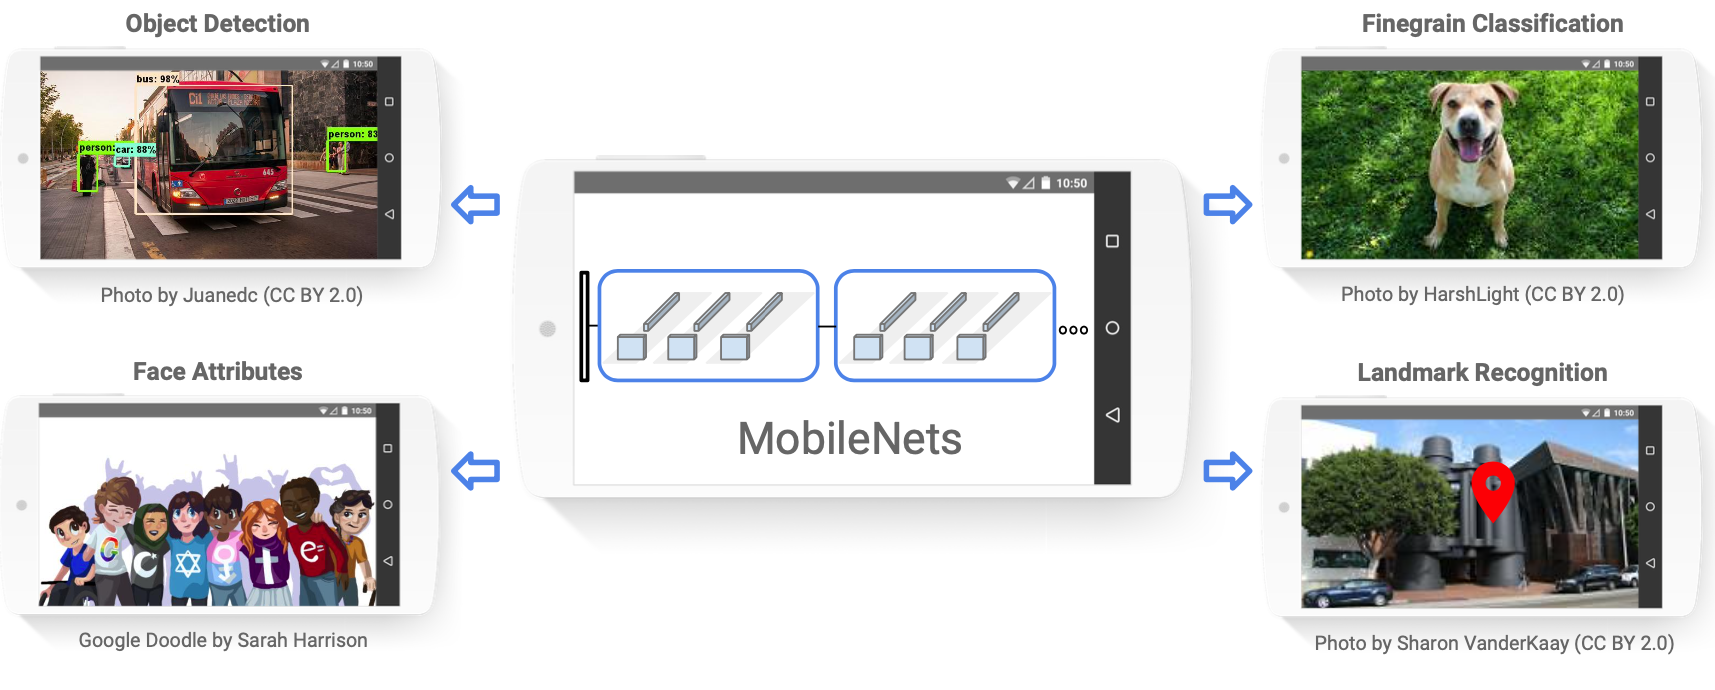
\includegraphics[width=\textwidth]{images/experiments/mobilenet_applications.png}
    \centering
    \caption{MobileNet applications}\label{fig:mobilenet_applications}
\end{figure}

Convolutional neural networks have been more popular in the recent years and
their accuracy increased thanks to more complex architecture increasing their
size whilst impacting negatively in speed. In many real world applications,
these networks need to run on edge devices with limited resources and the
inferences need to be carried out in a timely fashion.

The main focus of MobileNet is to increase the efficiency of the network by
decreasing the number of parameters by not compromising
performance\cite{review_mobilenet}.

\subsection{Depthwise Separable Convolution}
Depthwise separable convolution is the core basis of MobileNet architecture. It
is a \textbf{depthwise convolution followed by a pointwise convolution}.

A normal convolution is shown in \autoref{fig:convolution}

\begin{figure}[ht]
    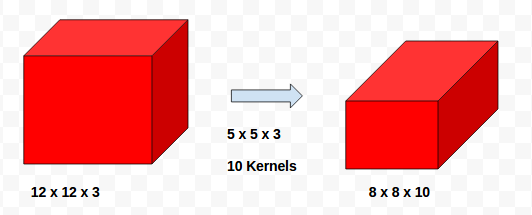
\includegraphics[width=10cm]{images/experiments/convolution.png}
    \centering
    \caption{Convolution}\label{fig:convolution}
\end{figure}

In the figure there is an input image size of $12\times12\times3$ and the
kernel (or filter) is $5\times5\times3$ with stride = 1. There are though 10
kernels to apply and this gives an output image of $8\times8\times10$.
The total computational cost is \bm{$12\times12\times5\times5\times3\times10 =
108000$}.

There are the following dimensions:
\begin{itemize}
    \item Input image: \bm{$D_f \times D_f \times M$}
    \item Output image: \bm{$D_f \times D_f \times N$}
    \item Convolution kernel: \bm{$D_k \times D_k \times M \times N$}
\end{itemize}

So in a normal convolution the total computational cost is
\bm{$D_k \times D_k \times M \times N \times D_f \times D_f$}

The above convolution can be divided  in 2 phases:
\begin{enumerate}
    \item Depthwise convolution
    \item Pointwise convolution
\end{enumerate}

The first one is the \textbf{depthwise convolution} and it is shown in
\autoref{fig:depthwise_convolution}.

\begin{figure}[ht]
    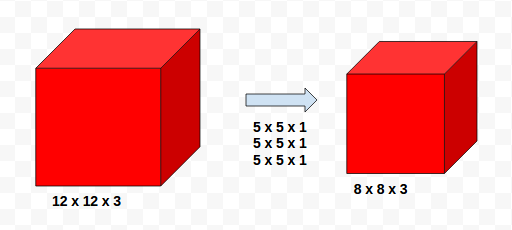
\includegraphics[width=10cm]{images/experiments/depthwise_convolution.png}
    \centering
    \caption{Depthwise convolution}\label{fig:depthwise_convolution}
\end{figure}

In this case the input has 3 channels and there are 3 $5\times5\times1$
kernels. These 3 kernels are applied to the three channels respectively
producing 3 $8\times8\times1$ output. When the 3 outputs are stacked the final
output is $8\times8\times3$.

The second phase is the \textbf{pointwise convolution} as shown in
\autoref{fig:pointwise_convolution}.

\begin{figure}[ht]
    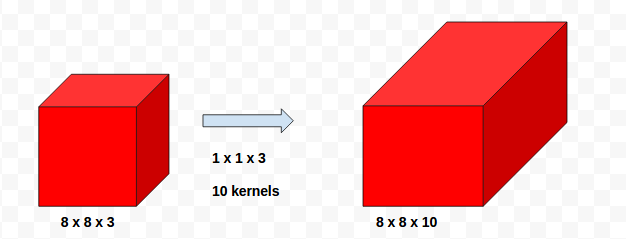
\includegraphics[width=10cm]{images/experiments/pointwise_convolution.png}
    \centering
    \caption{Pointwise convolution}\label{fig:pointwise_convolution}
\end{figure}

The output image of the previous step is the input image for this step.
The convolution is done using a $1\times1\times3$ kernel on the input image
producing a feature map. Repeating this using 10 different $1\times1\times3$
kernels will produce 10 different feature maps that will be stacked together.

The computation for each step is:
\begin{enumerate}
    \item Depthwise convolution: \bm{$12 \times 12 \times 5 \times 5 \times 3 =
        10800$}
    \item Pointwise convolution: \bm{$8 \times 8 \times 3 \times 10 = 1920$}
\end{enumerate}

Therefore the total number of computations is \textbf{10800 + 1920 = 12720}

More generically the computational cost is \bm{$D_k \times D_k \times M \times
D_f \times D_f + M \times N \times D_f \times D_f$}

In this specific case using a kernel of $3 \times 3$ there is about 8 to 9
times less computational reduction: \bm{$108000 / 12720 \approx 8.45$}

\subsection{MobileNet architecture}
The network architecture is built on depthwise separable convolutions except
for the first layer which is a full convolution

There are 28 convolutional layers (counting depthwise and pointwise layers) and
1 fully connected layer followed by a softmax layer
(\autoref{fig:mobilenet_architecture}).

\begin{figure}[ht]
    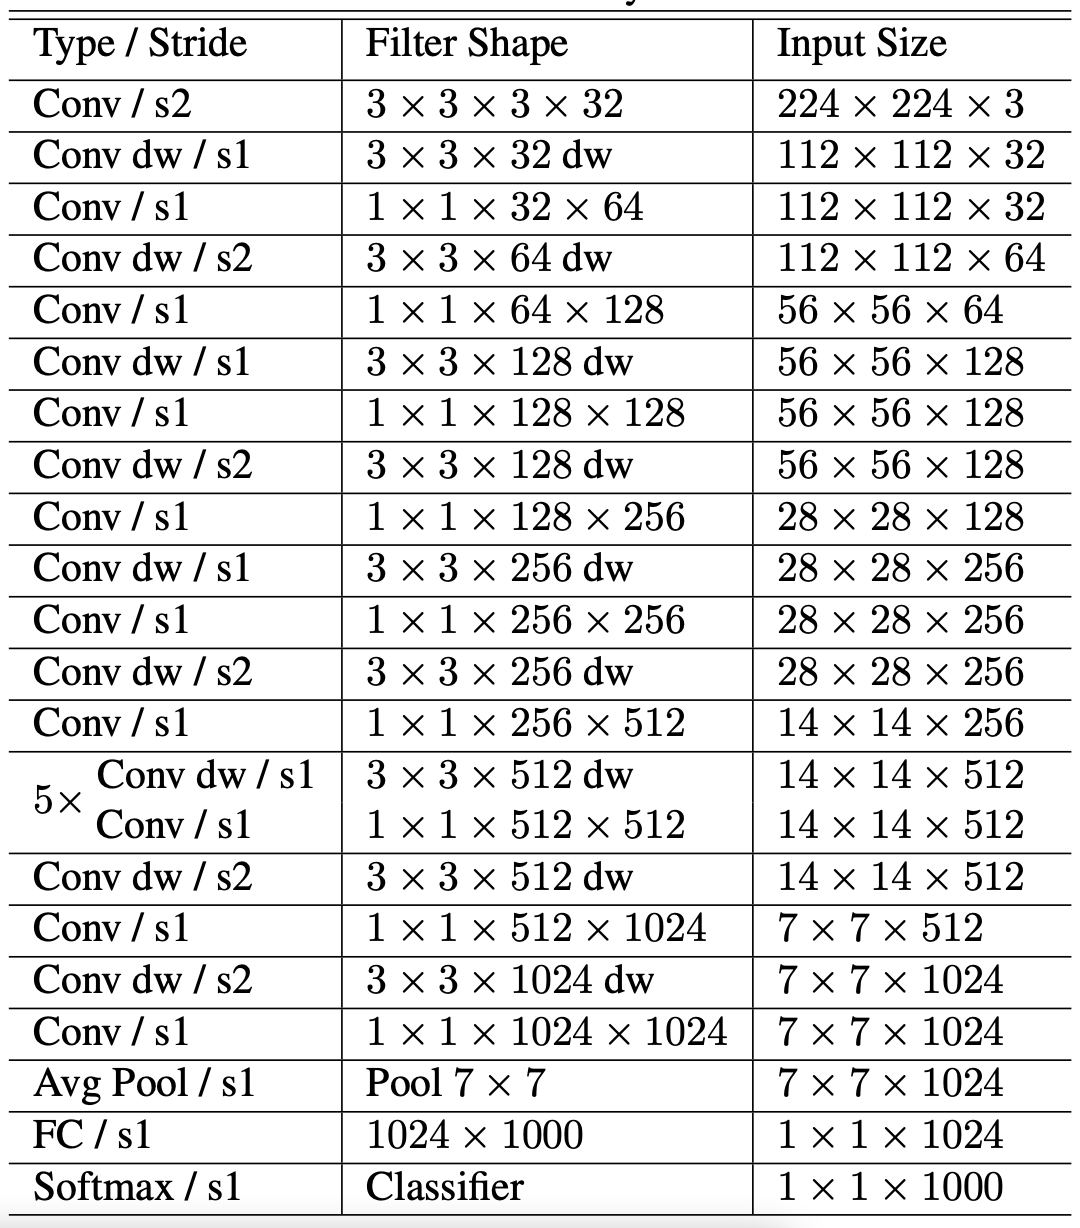
\includegraphics[width=10cm]{images/experiments/mobilenet_architecture.png}
    \centering
    \caption{MobileNet architecture}\label{fig:mobilenet_architecture}
\end{figure}

All layers are followed by a batch normalization and ReLU non linearity
(\autoref{fig:mobilenet_convolution}) with the exception of the final fully
connected layer which has no non linearity and feeds into a softmax layer for
classification.
As seen earlier in the thesis, the softmax is used to to predict a single class
of K mutually exclusive classes. In the case of MobileNet, when used with
ImageNet, it can classify up to 1000 classes.

\begin{figure}[ht]
    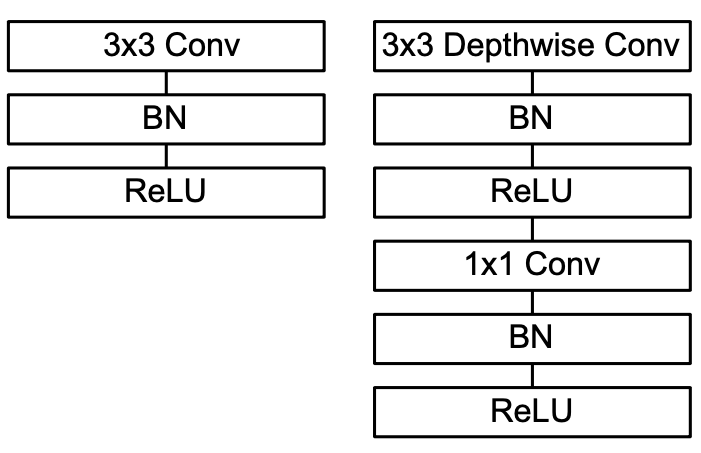
\includegraphics[width=8cm]{images/experiments/mobilenet_convolution.png}
    \centering
    \caption{Normal convolution vs MobileNet convolution}\label{fig:mobilenet_convolution}
\end{figure}

\subsection{Width Multiplier}
MobileNet has been developed to be small and low latency but sometimes specific
use cases or applications need the model to be faster and smaller.
In order to construct these smaller and less computationally expensive models
a very simple parameter \bm{$\alpha$} called width multiplier has been
introduced.

The role of the width multiplier $\alpha$ is to thin a network uniformly at
each layer: the number of input channels M becomes $\alpha M$ and the number of
output channels N becomes $\alpha N$.

So depth wise separable computational cost becomes \bm{$D_k \times D_k \times
\alpha M \times D_f \times D_f + \alpha M \times \alpha N \times D_f \times
D_f$} where $\alpha \in \interval[open left]{0}{1}$ with typical settings of 1,
0.75, 0.5, 0.25.

The \autoref{fig:mobilenet_widthmultiplier} shows the impact that $\alpha$ has
on accuracy, numbers of operations and parameters.

\begin{figure}[ht]
    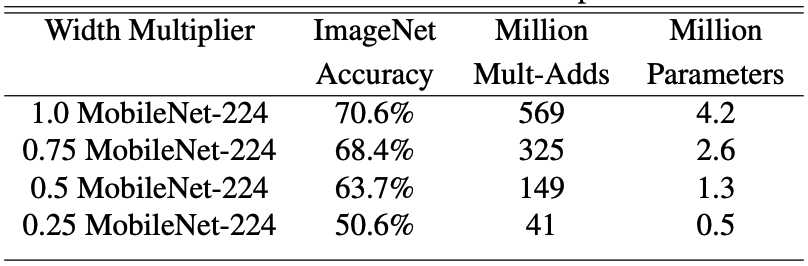
\includegraphics[width=10cm]{images/experiments/mobilenet_widthmultiplier.png}
    \centering
    \caption{Width multiplier impact}\label{fig:mobilenet_widthmultiplier}
\end{figure}

In this thesis I consider \bm{$\alpha = 1$} to be the baseline.

\subsection{Resolution Multiplier}
The second hyper-parameter to reduce the computational cost of a neural network
is a resolution multiplier \bm{$\rho$}. This can be applied to the input image
and the internal representation of every layer is subsequently reduced by the
same multiplier.
Including $\rho$, the computational cost becomes \bm{$D_k \times D_k \times
\alpha M \times \rho D_f \times \rho D_f + \alpha M \times \alpha N \times \rho
D_f \times \rho D_f$} where $\rho \in \interval[open left]{0}{1}$i which is
typically set implicitly so that the input resolution of the network is 224,
192, 160 or 128.

The \autoref{fig:mobilenet_resolutionmultiplier} shows the impact that $\rho$
has on accuracy, numbers of operations and parameters.

\begin{figure}[ht]
    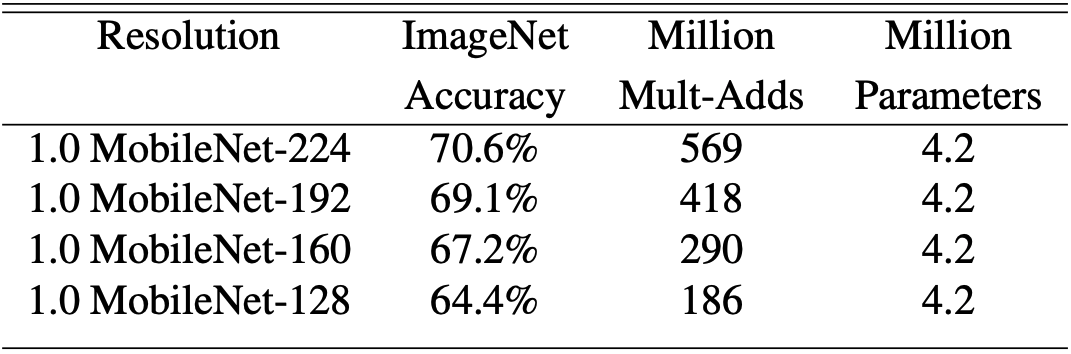
\includegraphics[width=10cm]{images/experiments/mobilenet_resolutionmultiplier.png}
    \centering
    \caption{Resolution multiplier impact}\label{fig:mobilenet_resolutionmultiplier}
\end{figure}

In this thesis I consider \bm{$\rho = 1$} to be the baseline.

\section{Datasets: CIFAR-10 and ImageNet}
In this section, I give a brief explanation of CIFAR-10 and ImageNet datasets.

\subsection{CIFAR-10 dataset}
The CIFAR-10 dataset (Canadian Institute For Advanced Research) is a collection
of images that are commonly used to train neural networks. It is one of the
most widely used datasets for machine learning research.

It consists of \textbf{60000} \bm{$32 \times 32$} colour images in
\textbf{10 classes}, with 6000 images per class. There are 50000 training
images and 10000 test images.

The dataset is divided into five training batches and one test batch, each with
10000 images. The test batch contains exactly 1000 randomly-selected images
from each class. The training batches contain the remaining images in random
order, but some training batches may contain more images from one class than
another. Between them, the training batches contain exactly 5000 images from
each class.

The 10 different classes represent airplanes, cars, birds, cats, deer, dogs,
frogs, horses, ships, and trucks (\autoref{fig:CIFAR_10}).

\begin{figure}[ht]
    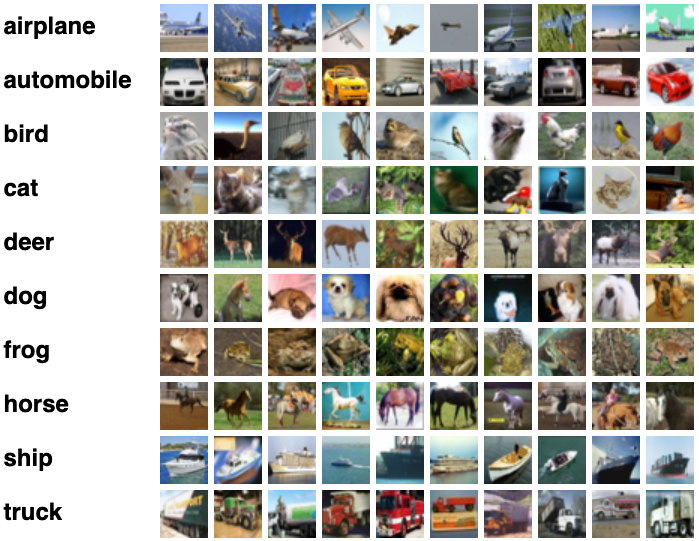
\includegraphics[width=\textwidth]{images/experiments/CIFAR_10.png}
    \centering
    \caption{CIFAR-10 sample images}\label{fig:CIFAR_10}
\end{figure}

The classes are completely mutually exclusive. There is no overlap between
automobiles and trucks. ``Automobile'' includes sedans, SUVs, things of that
sort. ``Truck'' includes only big trucks. Neither includes pick-up trucks.

\subsection{ImageNet 2012 dataset}
ImageNet is an image dataset organized according to the WordNet hierarchy. Each
meaningful concept in WordNet, possibly described by multiple words or word
phrases, is called a ``synonym set'' or ``synset''. There are more than 100000
synsets in WordNet, majority of them are nouns (80000+). In ImageNet, there are
on average 1000 images to illustrate each synset.
Images of each concept are quality-controlled and human-annotated. In its
completion, ImageNet will offer tens of millions of cleanly sorted images for
most of the concepts in the WordNet hierarchy (\autoref{fig:imagenet})

\begin{figure}[ht]
    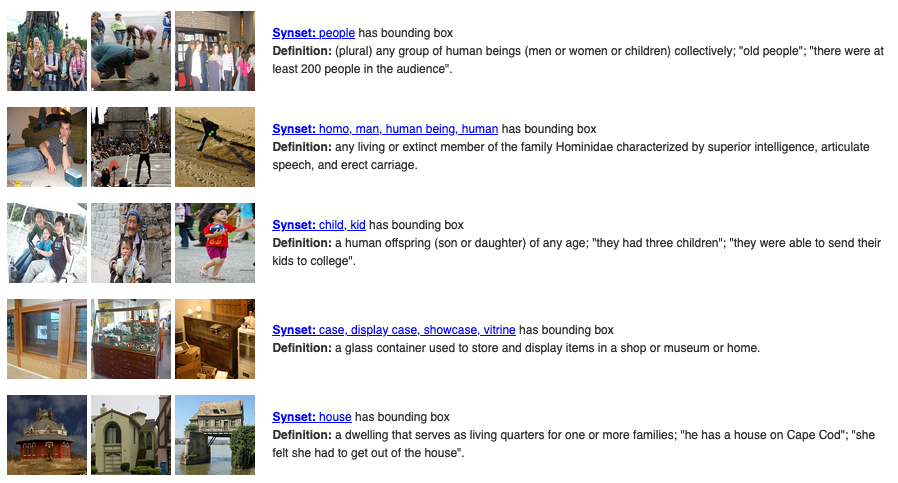
\includegraphics[width=\textwidth]{images/experiments/imagenet.png}
    \centering
    \caption{ImageNet sample images}\label{fig:imagenet}
\end{figure}

The dataset I've used for the experiments has the following sets:

\begin{itemize}
    \item \texttt{train} containing \textbf{1281167 images}
    \item \texttt{validation} containing \textbf{50000 images}
\end{itemize}

There supposed to be a \texttt{test} set but it doesn't have labels because no
labels have been publicly released.

The ILSVRC uses a ``trimmed'' list of only \textbf{1000 image categories} or
``classes'', including 90 of the 120 dog breeds classified by the full ImageNet
schema.

\section{Analysis of the experiment results}
After a brief explanation of the model and the datasets used for the
experiments, in this section I show what results I have in pruning MobileNet v1
with CIFAR-10 and ImageNet.

\subsection{Environments}
The environment used for running CIFAR-10 experiments has the following
characteristics:

\begin{itemize}
    \item \textbf{CPU and memory:} 2 x Intel Xeon Gold 5120T CPU @ 2.20GHz, 28
        cores (56 threads) total, 64GB memory
    \item \textbf{Graphic:} NVIDIA TITAN Xp, 12GB GDDR5X, 3840 cores, CUDA
        driver version: 460.27.04, CUDA version: 11.2
    \item \textbf{Operating System:} Ubuntu 18.04.5 LTS, kernel
        5.4.0\-60-generic
    \item \textbf{Software Stack:} Python 3.8.5, TensorFlow 2.4.0, TFMOT
        0.5.0.dev20210206 with my patch for heuristic distribution, and
        dependencies. Everything has been isolated using conda
        (\url{https://docs.conda.io/en/latest/})
\end{itemize}

The environment used for running ImageNet experiments has the following
characteristics:

\begin{itemize}
    \item \textbf{CPU and memory:} AWS p3.2xlarge, 8 vCPU, 61GB memory
    \item \textbf{Graphic:} NVIDIA Tesla V100, 16GB, 5120 cores, CUDA Driver
        Version: 450.80.02, CUDA Version: 11.0
    \item \textbf{Operating System:} Ubuntu 18.04.5 LTS, kernel
        5.4.0\-1037-aws
    \item \textbf{Software Stack:} Python 3.7.6, TensorFlow 2.4.1, TFMOT
        0.5.0.dev20210206 with my patch for heuristic distribution, and
        dependencies. Everything has been isolated using conda
        (\url{https://docs.conda.io/en/latest/})
\end{itemize}

The reason I chose AWS for ImageNet is because of the time the training takes
with this dataset: one epoch is about 1.5h and I needed to run 20 epochs.
As I show later, the number of experiments are 20 and AWS gives me the
flexibility to have multiple instances in parallel.

\subsection{Pipeline details}
In order to run experiments, I've developed a custom pipeline (not included in
this thesis) which executes the following steps:

\begin{enumerate}
    \item Load in memory the model architecture from a pre-trained checkpoint
    \item Convert the model into float32, int8 and int16 tflite format
    \item Prune the original model with given parameters
    \item Check model sparsity and calculate loss, TOP-1 and TOP-5 accuracies
    \item Convert the pruned model into float32, int8 and int16 tflite format
    \item For every tflite generated, run:
    \begin{enumerate}
        \item Accuracy evaluation on the validation dataset (10000 samples)
        \item Get the size and compressed size of the tflite file
        \item Only for int8/int16 tflite files: run Ethos-U vela
            (\autoref{sub:vela}) to get an estimation of the inference speed on
            Ethos-U NPU and the tflite size of the vela generated tflite file.
    \end{enumerate}
\end{enumerate}

The above pipeline has been run passing different sparsity level and
distributions. I ran 10 pipelines for every dataset: (Heuristic, 0.5),
(Uniform, 0.5), (Heuristic, 0.75), (Uniform, 0.75), (Heuristic, 0.8),
(Uniform, 0.8), (Heuristic, 0.85), (Uniform, 0.85), (Heuristic, 0.9),
(Uniform, 0.9).

The pruning scheduler chosen is \texttt{PolynomialDecay}: sparsity is
introduced slowly, model weights can take into account this impact and become
robust to the effect of weights being dropped.

Every run of the pipeline gives the following metrics:
\begin{enumerate}
    \item Keras model: loss, TOP-1 and TOP-5 accuracies
    \item For every tflite file: sizes of the original model, compressed, and
        pruned compressed
    \item For every int8/int16 tflite file: inference speed and vela compressed
        size
\end{enumerate}

Later I'll show graph that compares the above metrics across sparsity levels
and distributions.

\subsection{Ethos-U Vela}\label{sub:vela}
Vela is a tool used to compile a TensorFlow Lite for Microcontroller (tflite)
neural network model into an optimised version that can run on an embedded
system containing an Arm Ethos-U NPU\@.

In order to be accelerated by the Ethos-U NPU the network operators must be
quantised to either 8-bit (unsigned or signed) or 16-bit (signed).

The optimised model will contain TensorFlow Lite Custom operators for those
parts of the model that can be accelerated by the Ethos-U NPU\@. Parts of the
model that cannot be accelerated are left unchanged and will instead run on the
Cortex-M series CPU using an appropriate kernel (such as the Arm optimised
CMSIS-NN kernels).

After compilation the optimised model can only be run on an Ethos-U NPU
embedded system.

The tool will also generate performance estimates for the compiled model.

For more information about vela, please refer to PyPi home page
\url{https://pypi.org/project/ethos-u-vela/}

\subsubsection{Vela memory optimization}\label{subsub:vela_memory_optimization}
The Vela compiler also performs various memory optimizations to reduce both the
permanent (for example flash) and runtime (for example SRAM) memory
requirements.
One such technique for permanent storage is the compression of all the weights
in the model.

Another technique is cascading, which addresses the runtime memory usage.
Cascading reduces the maximum memory requirement by splitting the feature maps
(FM) of a group of consecutively supported operators into stripes. A stripe can
be either the full or partial width of the FM\@. And it can be the full or
partial height of the FM\@. Each stripe in turn is then run through all the
operators in the group.

The parts of the model that can be optimized and accelerated are grouped and
converted into TensorFlow Lite custom operators. The operators are then
compiled into a command stream that can be executed by the Ethos-U NPU\@.

Finally, the optimized model is written out as a $TFL\mu$ model and a
Performance Estimation report is generated that provides statistics, such as
memory usage and inference time.

The compiler includes numerous configuration options that allow you to specify
various aspects of the embedded system configuration (for example the Ethos-U
NPU configuration, memory types, and memory sizes). There are also options to
control the types of optimization that are performed during the compilation
process.\cite{vela_compiler}

\subsection{Results for MobileNet v1 with CIFAR-10}
For running this experiment the classical MobileNet v1 architecture has been
slightly modified on three layers.

\begin{figure}[ht]
    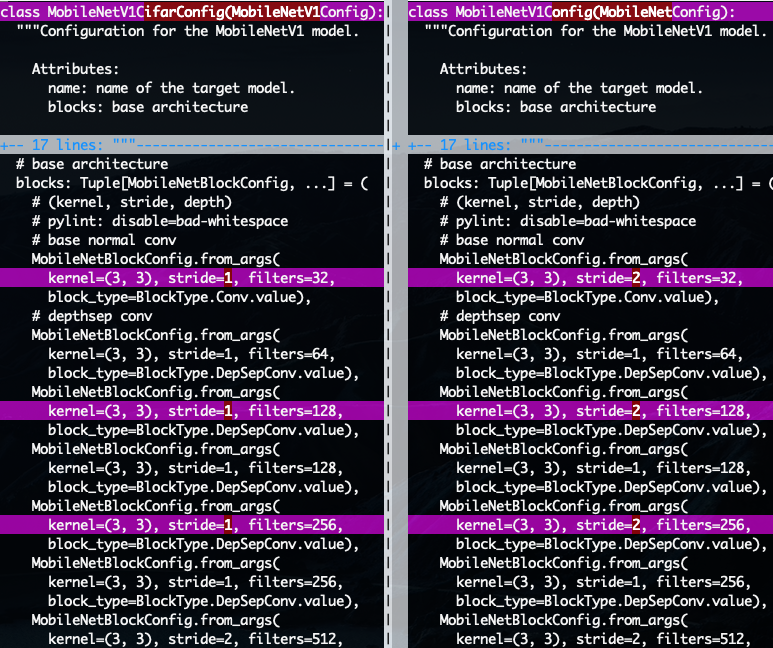
\includegraphics[width=9cm]{images/experiments/mobilenet_cifar10_diff.png}
    \centering
    \caption{MobileNet v1 changes for CIFAR-10}\label{fig:mobilenet_cifar10_diff}
\end{figure}

The original MobileNet architecture is designed for ImageNet dataset where
images' size is $224\times224\times3$. Because CIFAR-10 images have smaller
size ($32\times32$) I had to modify slightly the architecture.

The main change is that in the first layers the \texttt{stride=2} has been
replaced with \texttt{stride=1}.
\autoref{fig:mobilenet_cifar10_diff} shows what the difference is between
MobileNet for CIFAR-10 and the classical architecture.

The fine-tuning of the model has been done with the following hyper parameters
which have been found with Keras Tuner
(\url{https://keras-team.github.io/keras-tuner/}):

\begin{itemize}
    \item \textbf{Optimizer}: SGD (Stochastic Gradient Descend)
    \item \textbf{Optimizer momentum}: 0
    \item \textbf{Batch size}: 32
    \item \textbf{Learning rate}: 6.995e-06 (0.000006995)
    \item \textbf{Epochs}: 15
    \item \textbf{Sparsity scheduler}: Polynomial Decay
\end{itemize}

\subsubsection{Accuracy and loss results}
In this section I analyse data about accuracy and loss. The heuristic
distribution will be always compared to the uniform distribution.

For reference, \textbf{the TOP-1 accuracy of a non-pruned MobileNet v1 with
CIFAR-10 is 0.9487.}

\autoref{fig:cifar10_top1_top5_loss} shows how the two distributions impact the
TOP-1/TOP-5 accuracies and the loss function.

\begin{figure}
    \centering
    {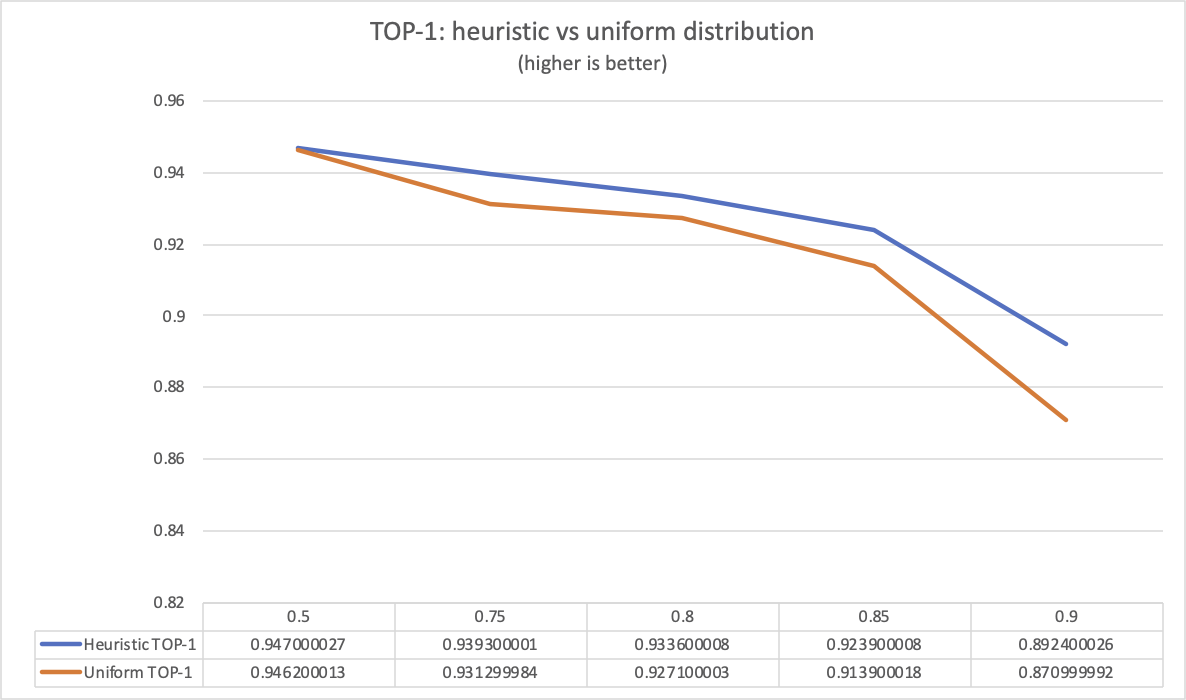
\includegraphics[width=.85\linewidth]{images/experiments/cifar10_top1.png}}
    {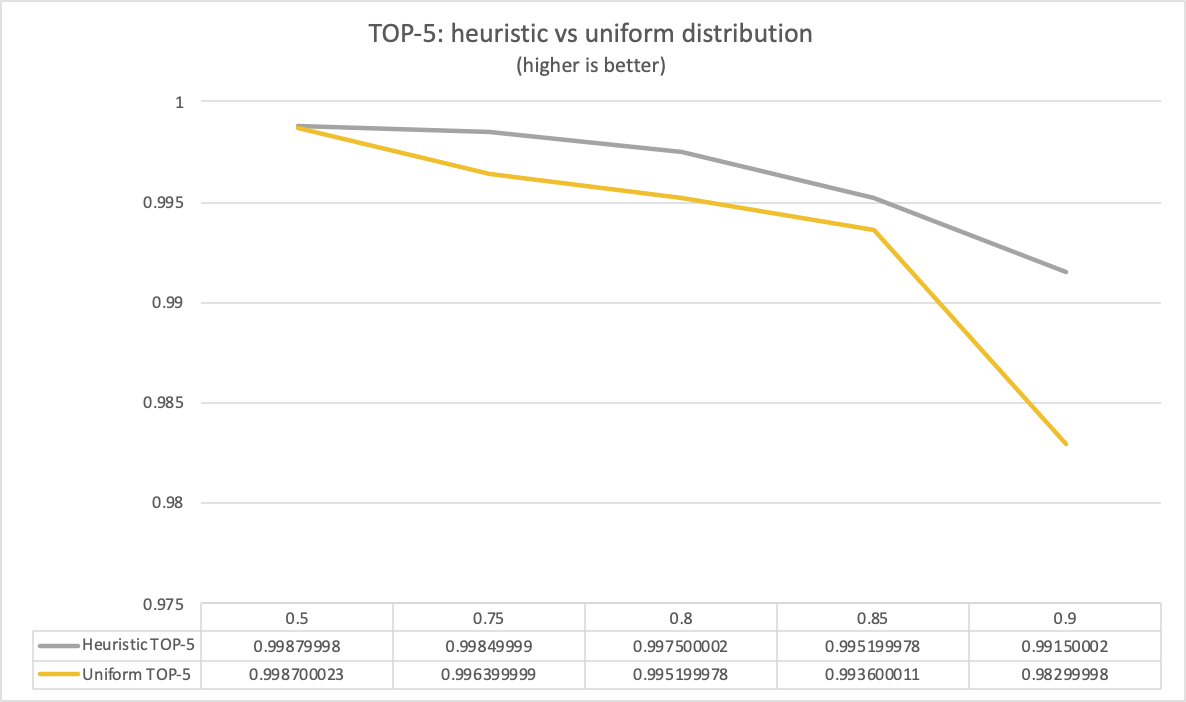
\includegraphics[width=.85\linewidth]{images/experiments/cifar10_top5.png}}
    {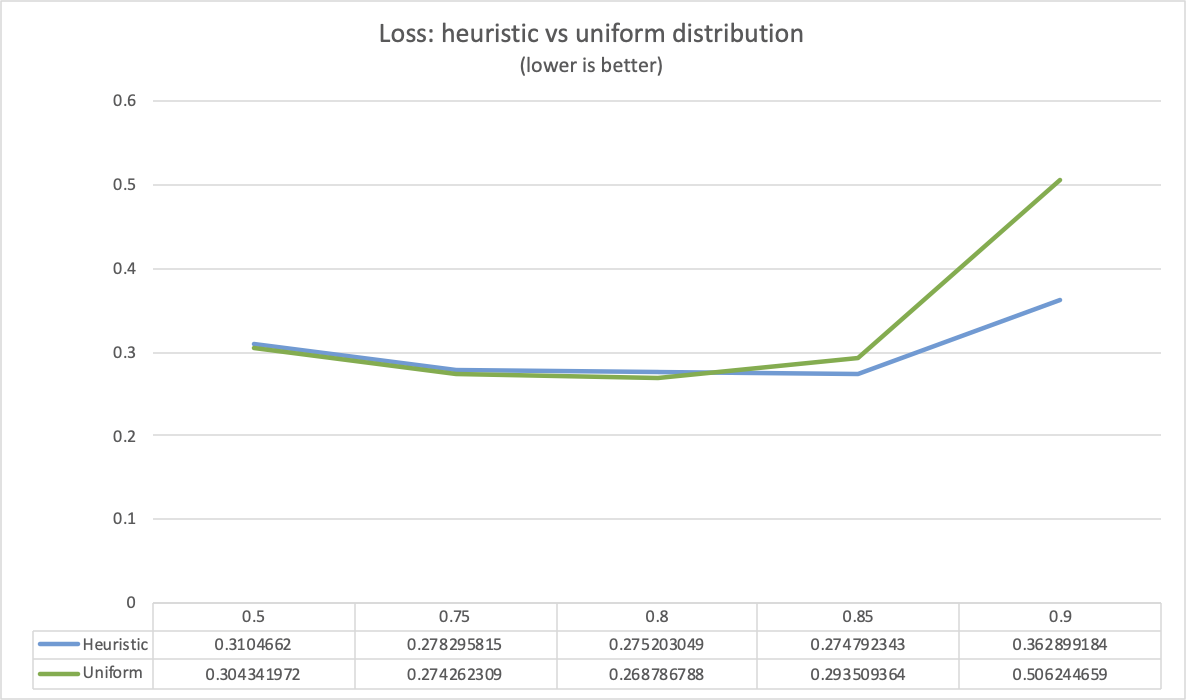
\includegraphics[width=.85\linewidth]{images/experiments/cifar10_loss.png}}
    \caption{Heuristic vs Uniform: CIFAR-10 TOP-1/TOP-5 and Loss}\label{fig:cifar10_top1_top5_loss}
\end{figure}

The first thing to notice is that the heuristic distribution always outperforms
the uniform distribution both for TOP-1 (blue line) and TOP-5 (grey line).
The heuristic distribution seems more robust compared to the uniform and this
is highlighted by the fact it loses less in accuracy when the sparsity is
increasing.
When the sparsity is set to 0.9, the heuristic distribution has an increase of
\textbf{2.14\% in the TOP-1} compared to the uniform distribution.
A sweet spot though is at \textbf{sparsity 0.85}: the model doesn't lose too
much accuracy compared to its non-pruned baseline and the sparsity is high
enough to see benefits in terms of size, memory and latency of the inference.
At this sparsity level, the heuristic distributions gains 1\% in accuracy
compared to the uniform distribution, giving an accuracy of \textbf{0.9239\%}:
this is \textbf{only 2.48\% less} than the non-pruned accuracy.

The loss has a slightly different trend: up to a sparsity level of 0.8, there
is no big difference between the two distributions with the uniform being
slightly better.
The trend completely flips at the latest two highest sparsity level: the loss
of the uniform distribution increases much more compared to the heuristic one.
This is another proof that the heuristic distribution seems more robust at
higher sparsity levels.

\begin{figure}[ht]
    \centering
    {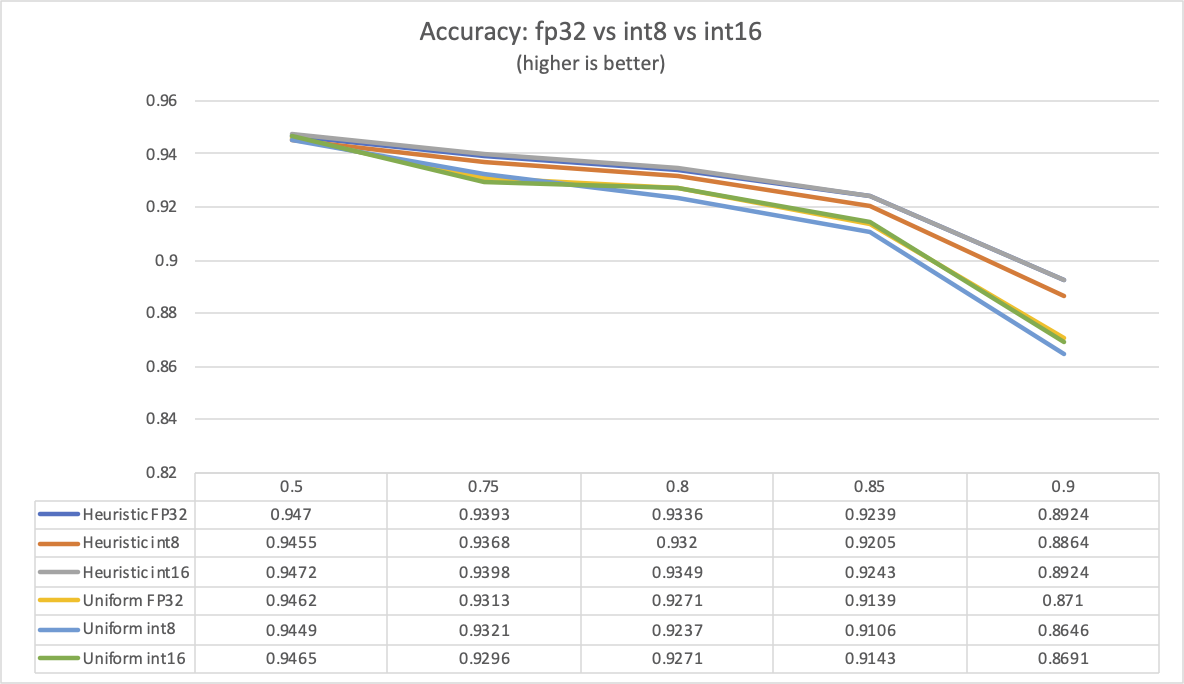
\includegraphics[width=.8\linewidth]{images/experiments/cifar10_tflite_accuracy.png}}
    \caption{Heuristic vs Uniform: CIFAR-10 tflite accuracy}\label{fig:cifar10_tflite_accuracy}
\end{figure}

\autoref{fig:cifar10_tflite_accuracy} shows accuracy across FP32, int8 and
int16 tflite models both for uniform and heuristic distribution.

This graph confirms the trend seen in the previous ones: independently of the
quantization scheme used, \textbf{the heuristic distribution performs better
than the uniform one across all sparsity levels}.
The top 3 lines (dark blue, amber and grey) represent the accuracies of the
heuristic distribution whilst the bottom 3 lines (yellow, light blue and green)
represent the accuracies of the uniform distribution.
Moreover the heuristic distribution seems to have a smoother trend across
sparsity levels compared to the uniform distribution.

\subsubsection{tflite size results}\label{subsub:tflite_size_results}
\autoref{fig:cifar10_tflite_size} shows the sizes of tflite files across
different sparsity levels for FP32, int8 and int16.

\begin{figure}[ht]
    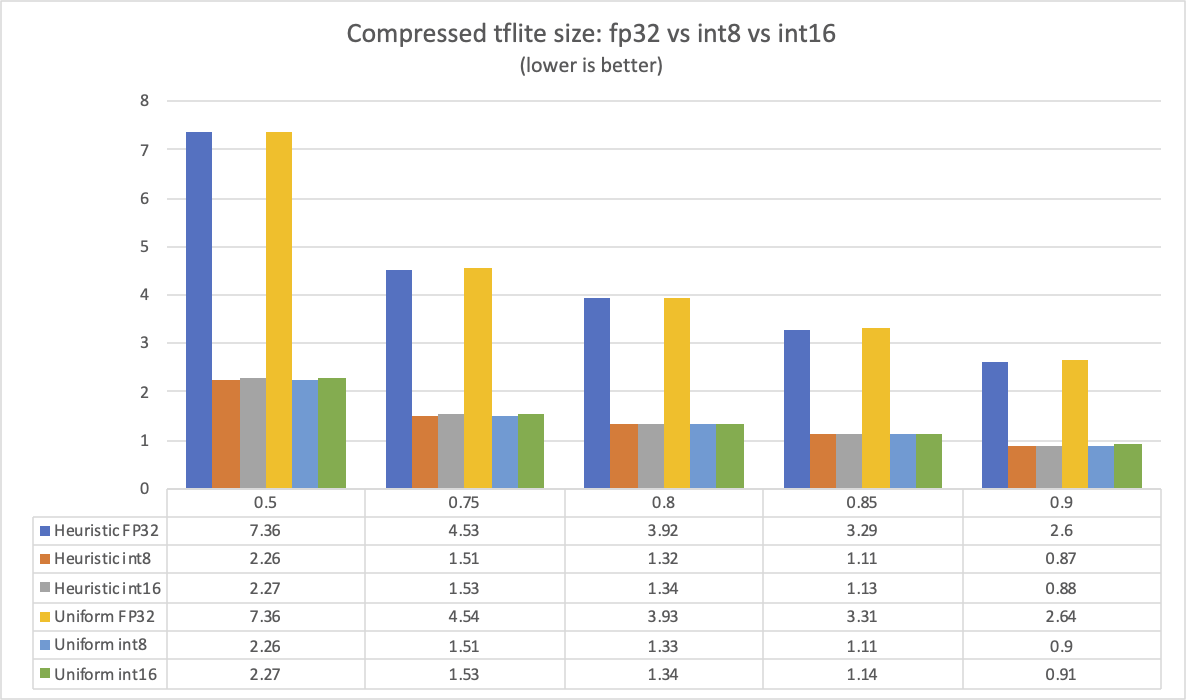
\includegraphics[width=\linewidth]{images/experiments/cifar10_tflite_size.png}
    \centering
    \caption{Heuristic vs Uniform: CIFAR-10 FP32, int8, int16 tflite size}\label{fig:cifar10_tflite_size}
\end{figure}

The sparsity distribution doesn't really influence the size of the tflite:
the distribution controls how weights are distributed across layers while
maintaining the final sparsity of the model. \textbf{The number of weights is
exactly the same.}
As example let's take the 0.85 sparsity level and see how the weights are
distributed in both heuristic and uniform distribution.

\begin{lstlisting}[label={lst:heuristic_weights_cifar10},
    caption=MobileNet v1 and CIFAR-10: heuristic weights distributions]
Conv2d_0_0:            864 weights,     384 zero weights,    0.4444444444444444 sparsity
Conv2d_1/pointwise:    2048 weights,    1026 zero weights,   0.5009765625 sparsity
Conv2d_2/pointwise:    8192 weights,    4851 zero weights,   0.5921630859375 sparsity
Conv2d_3/pointwise:    16384 weights,   10448 zero weights,  0.6376953125 sparsity
Conv2d_4/pointwise:    32768 weights,   22388 zero weights,  0.6832275390625 sparsity
Conv2d_5/pointwise:    65536 weights,   47760 zero weights,  0.728759765625 sparsity
Conv2d_6/pointwise:    131072 weights,  101490 zero weights, 0.7743072509765625 sparsity
Conv2d_7/pointwise:    262144 weights,  214920 zero weights, 0.819854736328125 sparsity
Conv2d_8/pointwise:    262144 weights,  214920 zero weights, 0.819854736328125 sparsity
Conv2d_9/pointwise:    262144 weights,  214920 zero weights, 0.819854736328125 sparsity
Conv2d_10/pointwise:   262144 weights,  214920 zero weights, 0.819854736328125 sparsity
Conv2d_11/pointwise:   262144 weights,  214920 zero weights, 0.819854736328125 sparsity
Conv2d_12/pointwise:   524288 weights,  453721 zero weights, 0.8654041290283203 sparsity
Conv2d_13/pointwise:   1048576 weights, 955202 zero weights, 0.9109516143798828 sparsity
top/Conv2d_1x1_output: 10250 weights,   6213 zero weights,   0.6061463414634146 sparsity
Sparse weights: 2678083
All weights: 3150698
Overall model sparsity: 0.8499967309
\end{lstlisting}

As shown in \autoref{lst:heuristic_weights_cifar10}, the heuristic distribution
of the weights has set to zero about 91\% of the weights in the layer
\texttt{Conv2d\_13/pointwise} while the first layers of the model have a
sparsity below 50\%.

For reference, \autoref{lst:uniform_weights} shows the same sparsity level
(0.85) but with a uniform distribution. All layers have 85\% of the weights set
to zero.

\begin{lstlisting}[label={lst:uniform_weights},
    caption=MobileNet v1 and CIFAR-10: uniform weights distributions]
Conv2d_0_0:            864 weights,    734 zero weights,    0.8495370370370371 sparsity
Conv2d_1/pointwise:    2048 weights,   1741 zero weights,   0.85009765625 sparsity
Conv2d_2/pointwise:    8192 weights,   6963 zero weights,   0.8499755859375 sparsity
Conv2d_3/pointwise:    16384 weights,  13926 zero weights,  0.8499755859375 sparsity
Conv2d_4/pointwise:    32768 weights,  27853 zero weights,  0.850006103515625 sparsity
Conv2d_5/pointwise:    65536 weights,  55706 zero weights,  0.850006103515625 sparsity
Conv2d_6/pointwise:    131072 weights, 111411 zero weights, 0.8499984741210938 sparsity
Conv2d_7/pointwise:    262144 weights, 222822 zero weights, 0.8499984741210938 sparsity
Conv2d_8/pointwise:    262144 weights, 222822 zero weights, 0.8499984741210938 sparsity
Conv2d_9/pointwise:    262144 weights, 222822 zero weights, 0.8499984741210938 sparsity
Conv2d_10/pointwise:   262144 weights, 222822 zero weights, 0.8499984741210938 sparsity
Conv2d_11/pointwise:   262144 weights, 222822 zero weights, 0.8499984741210938 sparsity
Conv2d_12/pointwise:   524288 weights, 445645 zero weights, 0.8500003814697266 sparsity
Conv2d_13/pointwise:   1048576 weights,891290 zero weights, 0.8500003814697266 sparsity
top/Conv2d_1x1_output: 10250 weights,  8704 zero weights,   0.849170731707317 sparsity
Sparse weights: 2678083
All weights: 3150698
Overall model sparsity: 0.8499967309
\end{lstlisting}

What the \autoref{fig:cifar10_tflite_size} highlights though is that quantized
models have a much smaller size compared to FP32.

As reference, the uncompressed version of the tflite files are:
\begin{itemize}
    \item \textbf{FP32}: 12.85Mb
    \item \textbf{int8}: 3.61Mb
    \item \textbf{int16}: 3.65Mb
\end{itemize}

At 0.85 sparsity level, there are the following gains in terms of sizes:
\begin{itemize}
    \item \textbf{FP32}: 12.85Mb $\rightarrow$ 3.30Mb, a \textbf{decrease of 74.31\%}
    \item \textbf{int8}: 3.61Mb $\rightarrow$ 1.11Mb, a \textbf{decrease of 69.25\%}
    \item \textbf{int16}: 3.65Mb $\rightarrow$ 1.13, a \textbf{decrease of 69.04\%}
\end{itemize}

As mentioned in \autoref{subsub:vela_memory_optimization}, vela compiler has a
compression mechanism built it when parsing a tflite file. In fact vela
generates a new tflite file which has a better compression rate compared to
gzip. Let's take the above sparsity level (0.85) and see how vela compiler
affects the tflite size. Of course this is true \textbf{only for quantized
tflite models.}
The non pruned quantized models (both int8 and int16) have a \textbf{vela size
of 3Mb.}. The pruned ones have a \textbf{vela size of 0.91Mb}, a \textbf{a
decrease of 69.67\%}.

Let's take the 2 extreme points of the tflite sizes: FP32 non pruned and
int8/int16 pruned at 0.85. \textbf{The tflite size goes from 12.85 to 0.91Mb,
a decrease of 92.92\%}. The accuracy goes from 0.9487 to 0.9205
(int8) or 0.9243 (int16), \textbf{a decrease of 2.97\% (int8) or 2.57\% (int16)}

\subsubsection{Inference speed results (int8 and int16 only)}
The inference speed showed in \autoref{fig:cifar10_inf_speed} are generated by
vela while optimising the tflite file. Vela compiler can take multiple profiles
depending for what NPU it needs to optimise the tflite for.

\begin{figure}
    \centering
    \subcaptionbox{Inference speed}
    {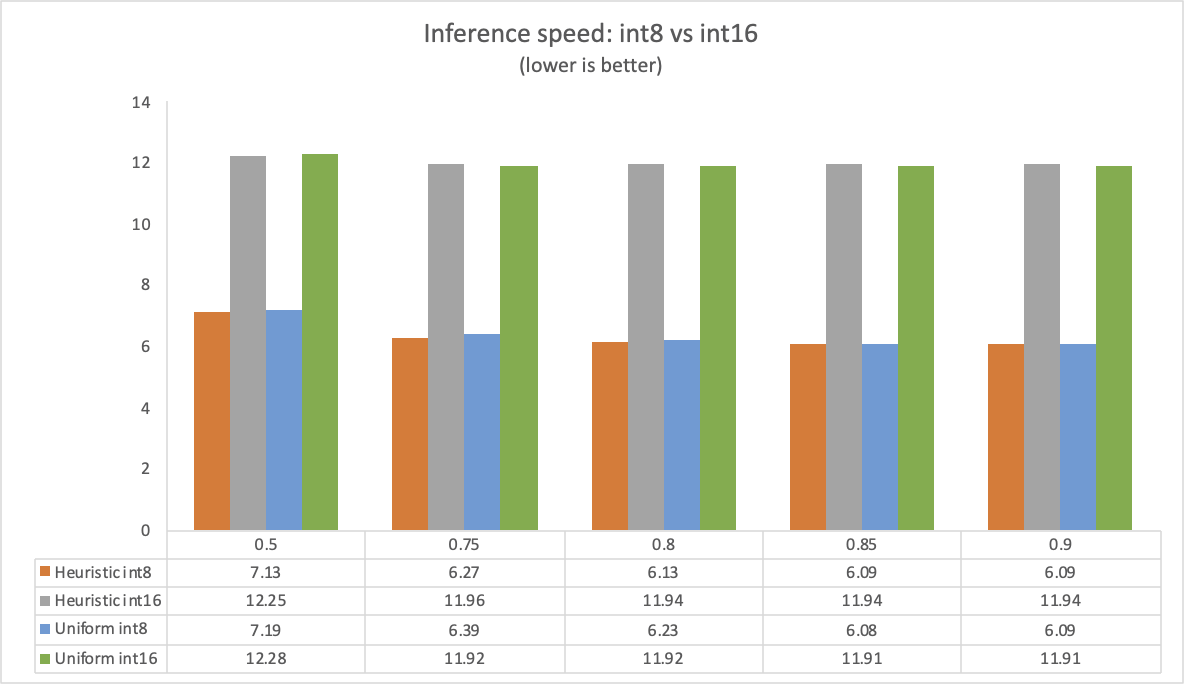
\includegraphics[width=1\linewidth]{images/experiments/cifar10_inf_speed.png}}
    \subcaptionbox{Inferences per second}
    {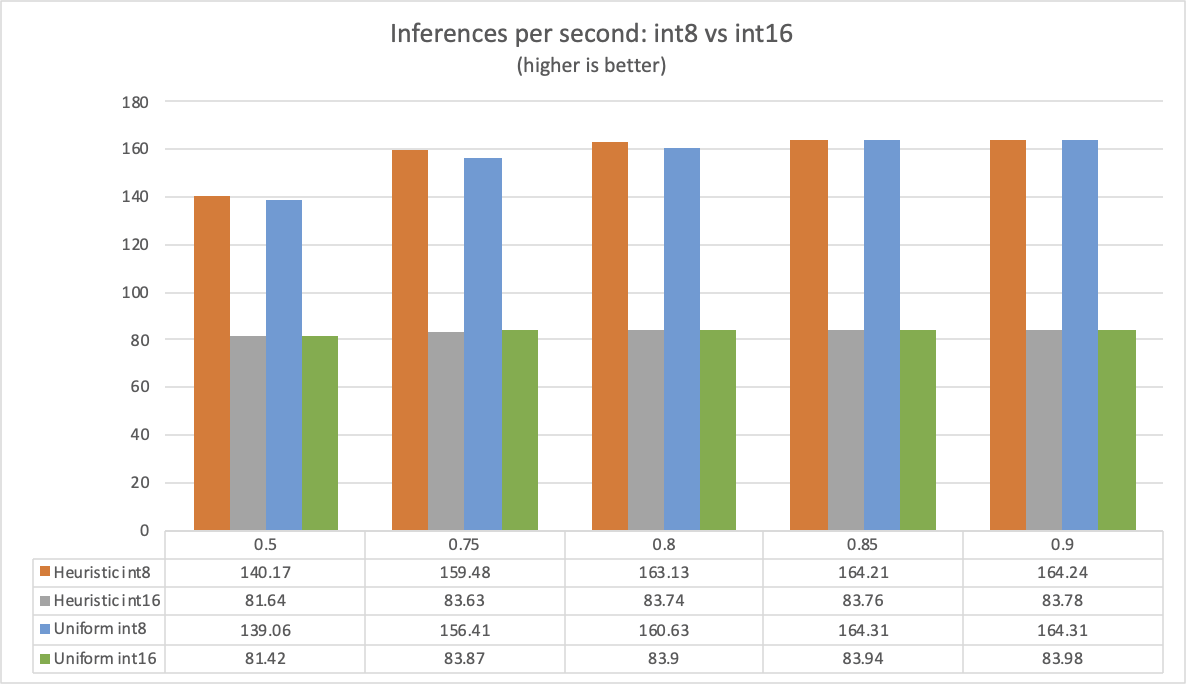
\includegraphics[width=1\linewidth]{images/experiments/cifar10_infs_second.png}}
    \caption{Heuristic vs Uniform: CIFAR-10 int8, int16 inference speed}\label{fig:cifar10_inf_speed}
\end{figure}

In this case the it has been optimised for an Ethos-U55 high-end embedded NPU
with the following characteristics: SRAM, 4 GB/s and flash, 0.5 GB/s.
\autoref{lst:vela_output_cifar10} shows vela output with estimations. At the very end
there is the inference speed (\texttt{Batch Inference time})

\begin{lstlisting}[label={lst:vela_output_cifar10},
    caption=MobileNet v1 and CIFAR-10: vela output on an int8 tflite file]
Warning: Using internal-default values for memory mode
Info: MEAN model_2/top/GlobalPool/Mean is a CPU only op
Warning: Mean operation is unknown or unsupported, placing on CPU

Network summary for mobilenet-v1_cifar10-int8-pruned
Accelerator configuration               Ethos_U55_256
System configuration             Ethos_U55_High_End_Embedded
Memory mode                          internal-default
Accelerator clock                                 500 MHz
Design peak SRAM bandwidth                       4.00 GB/s
Design peak Off-chip Flash bandwidth             0.50 GB/s

Total SRAM used                                415.64 KiB
Total Off-chip Flash used                      899.83 KiB (2.20 bits per element)

69 passes fused into 58
1/191 (52.4%) operations falling back to the CPU
Average SRAM bandwidth                           2.82 GB/s
Input   SRAM bandwidth                           7.71 MB/batch
Weight  SRAM bandwidth                           6.19 MB/batch
Output  SRAM bandwidth                           3.25 MB/batch
Total   SRAM bandwidth                          17.19 MB/batch
Total   SRAM bandwidth            per input     17.19 MB/inference (batch size 1)

Average Off-chip Flash bandwidth                 0.14 GB/s
Input   Off-chip Flash bandwidth                 0.11 MB/batch
Weight  Off-chip Flash bandwidth                 0.77 MB/batch
Output  Off-chip Flash bandwidth                 0.00 MB/batch
Total   Off-chip Flash bandwidth                 0.88 MB/batch
Total   Off-chip Flash bandwidth  per input      0.88 MB/inference (batch size 1)

Neural network macs                         611565578 MACs/batch
Hardware macs                               668484736 MACs/batch
Network Tops/s                                   0.20 Tops/s
Hardware Tops/s                                  0.22 Tops/s

NPU cycles                                    2967787 cycles/batch
SRAM Access cycles                            2148562 cycles/batch
DRAM Access cycles                                  0 cycles/batch
On-chip Flash Access cycles                         0 cycles/batch
Off-chip Flash Access cycles                   881088 cycles/batch
Total cycles                                  3044776 cycles/batch

Batch Inference time                 6.09 ms,  164.22 inferences/s (batch size 1)
\end{lstlisting}

Similarly to what has been observed in \autoref{subsub:tflite_size_results},
the distribution doesn't really impact the inference speed.
It looks like though that the heuristic distributions is slightly faster than
the uniform one but the increase is so small that can be ignored.

\autoref{fig:cifar10_inf_speed} shows anyway that int16 is much slower than
int8: this because the native MACs (multiply-accumulate) operations in
Ethos-U55 are 8 (for weights) $\times$ 8 (for activations) bit.
8$\times$16-bit operations run at half the speed of 8$\times$8-bit
operations as a 8$\times$16 MAC is twice as complex as an 8$\times$8 MAC\@.

Let's take the inference time for non-pruned tflite files and see what kind of
speed up there is with a pruned model at 0.85.

\begin{itemize}
    \item \textbf{int8}: 8.68ms $\rightarrow$ 6.09ms, a \textbf{decrease of 29.84\%}
    \item \textbf{int16}: 13.93ms $\rightarrow$ 11.91ms, a \textbf{decrease of 14.50\%}
\end{itemize}

Quantization has a huge benefit in terms of tflite size and latency of the
inference and the benefits are even bigger when paired up with pruning.

\subsection{Results MobileNet v1 with ImageNet 2012}
After seen the results using CIFAR-10, in this section the dataset used is
ILSVRC (ImageNet Large Scale Visual Recognition Challenge) 2012, commonly known
as ImageNet.

There are no architectural changes to the model.

The fine-tuning of the model has been done with the following hyper parameters
found via experimentations:

\begin{itemize}
    \item \textbf{Optimizer}: SGD (Stochastic Gradient Descend)
    \item \textbf{Optimizer momentum}: 0.9
    \item \textbf{Optimizer decay rate}: 0.9
    \item \textbf{Learning rate decay rate}: 0.94
    \item \textbf{Learning rate decay epochs}: 2.5
    \item \textbf{Dropout rate}: 0.2
    \item \textbf{Standard weight decay}: 4e-05
    \item \textbf{Truncated normal standard deviation}: 0.09
    \item \textbf{Batch norm decay}: 0.9997
    \item \textbf{Batch size}: 64
    \item \textbf{Learning rate}: 0.001
    \item \textbf{Epochs}: 20
    \item \textbf{Sparsity scheduler}: Polynomial Decay
\end{itemize}

\subsubsection{Accuracy and loss results}
For ImageNet I focus mainly on the FP32 results as similar considerations to
CIFAR-10 can be done for quantized models in terms of accuracy.

Like before, the heuristic distribution will be always compared to the uniform
distribution.

For reference, \textbf{the TOP-1 accuracy of a non-pruned MobileNet v1 with
ImageNet is 0.709.}

\autoref{fig:imagenet_top1_top5_loss} shows how the two distributions impact the
TOP-1/TOP-5 accuracies and the loss function.

\begin{figure}
    \centering
    {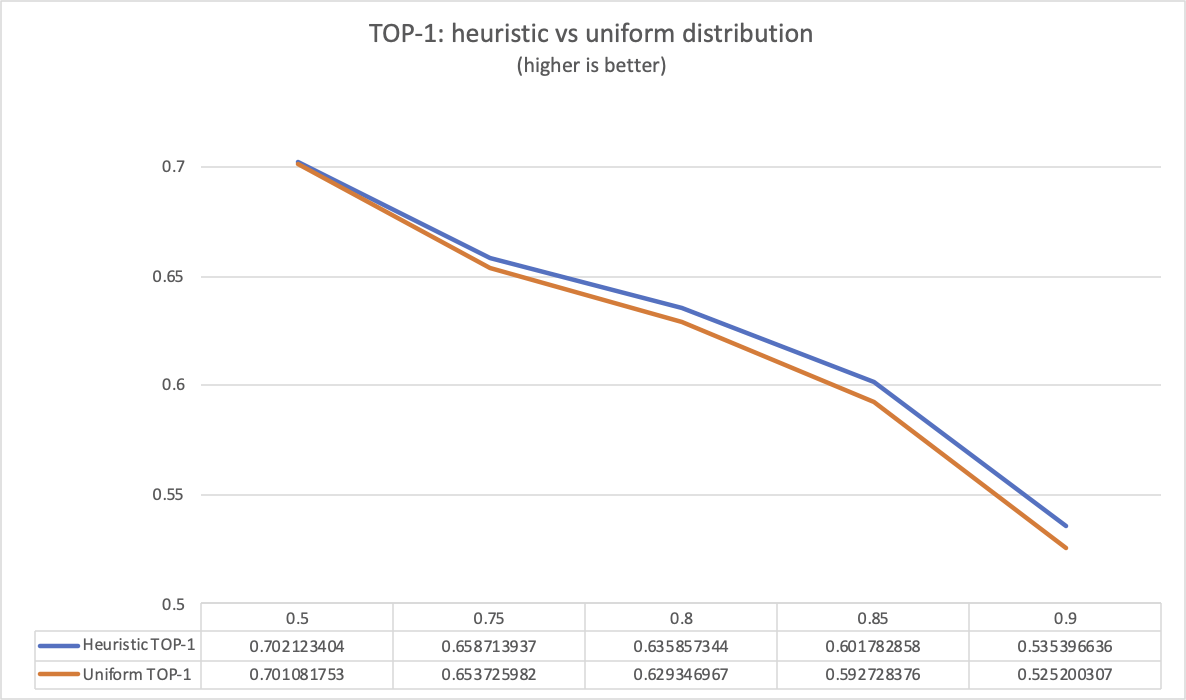
\includegraphics[width=.85\linewidth]{images/experiments/imagenet_top1.png}}
    {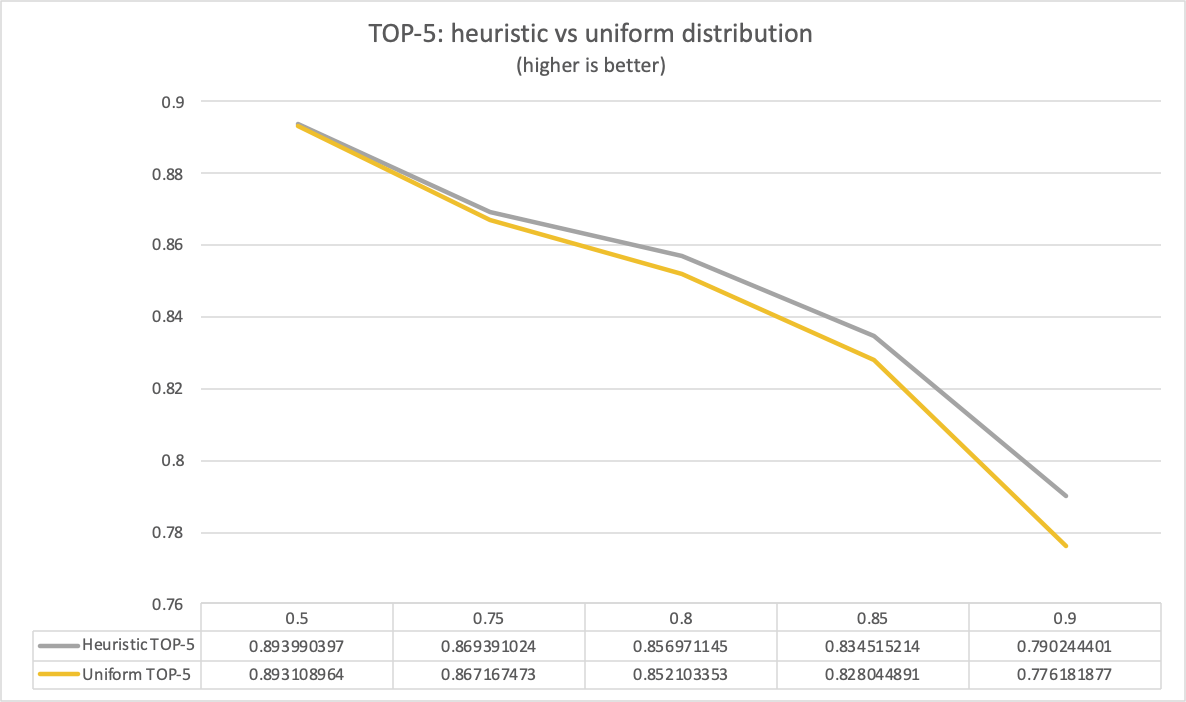
\includegraphics[width=.85\linewidth]{images/experiments/imagenet_top5.png}}
    {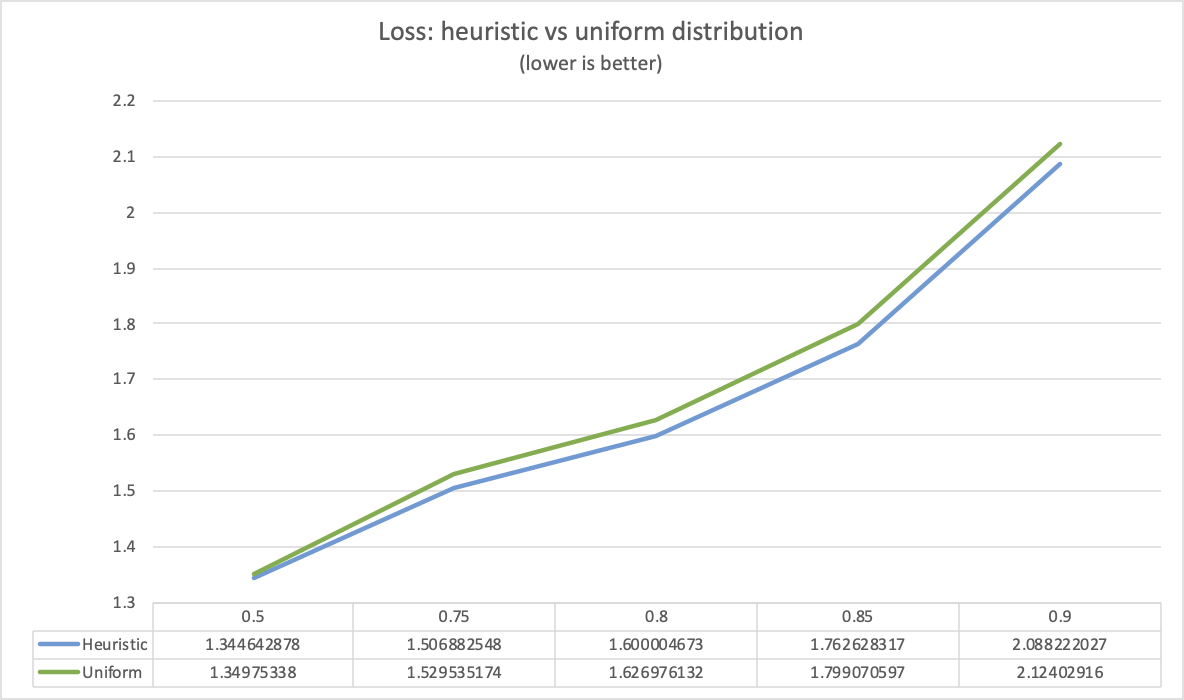
\includegraphics[width=.85\linewidth]{images/experiments/imagenet_loss.png}}
    \caption{Heuristic vs Uniform: ImageNet TOP-1/TOP-5 and Loss}\label{fig:imagenet_top1_top5_loss}
\end{figure}

Like in the previous case, the heuristic distribution always outperforms the
uniform distribution both for TOP-1 (blue line) and TOP-5 (grey line).
The heuristic distribution seems more a little bit more robust compared to the
uniform one as the sparsity increases the difference between the two sparsity
increases slightly.
When the sparsity is set to 0.9, the heuristic distribution has an increase of
\textbf{1.02\% in the TOP-1} compared to the uniform distribution.
\textbf{Any sparsity bigger than 0.5 is going to have an impact in terms of
accuracy}: the TOP-1 accuracy for a non pruned model is 0.709 and for a
sparsity of 0.5 there is a TOP-1 accuracy of 0.7021 for the heuristic
distribution and 0.7011 for the uniform distribution.
If the requirements of the application need to have a close accuracy of the
original model, then 0.5 is a pretty good sparsity level. At this point
choosing one of the other distribution changes very little in terms of
accuracy: the heuristic has only \textbf{0.1041\%} more accuracy than the
uniform distribution.
If the application requires a smaller model, it needs to compromise in the
accuracy: from 0.75 to 0.85 sparsity level, there is a drop of about 6\%.
At 0.85 sparsity level, the heuristic distribution has an accuracy of
\textbf{0.6018} whilst the uniform distributions falls in the range below, at
\textbf{0.5927}.
At 0.9 sparsity level there is a steeper drop in accuracy (around 0.52): with
this accuracy it might not make any sense to deploy the model at all.
If the sparsity needs to be between 0.5 and 0.85 then the heuristic
distribution is the one of choice as it gives better accuracy.

The loss follows has a specular behaviour of the TOP-1 accuracy: at 0.5
sparsity level the loss function is the same for both distribution.
From 0.75 to 0.85 they increase almost in a parallel fashion and to get to 0.9
were both distributions have a steeper increase.
Anyway from 0.75 to 0.9 the heuristic distribution (blue line) has always a
smaller loss function compared to the uniform.
This is another proof that the heuristic distribution seems more robust at
higher sparsity levels.

\subsubsection{tflite size results}
Like in the previous case, the sparsity distribution doesn't really influence
the size of the tflite: the number of weights is exactly the same between the
uniform and the heuristic distributions.

This model though is bigger than the previous one: even the architecture is the
same, it deals with different input size: CIFAR-10 images are 32$\times$32
whilst ImageNet images are 224$\times$224.

Let's take the 0.85 sparsity level and see how the weights are distributed
following the heuristic distribution.

\begin{lstlisting}[label={lst:heuristic_weights_imagenet},
    caption=MobileNet v1 and ImageNet: heuristic weights distributions]
2021-02-19 15:26:23,484 Conv2d_0_0:            864 weights,     377 zero weights,    0.4363425925925926 sparsity
2021-02-19 15:26:23,488 Conv2d_1/pointwise:    2048 weights,    1008 zero weights,   0.4921875 sparsity
2021-02-19 15:26:23,492 Conv2d_2/pointwise:    8192 weights,    4765 zero weights,   0.5816650390625 sparsity
2021-02-19 15:26:23,496 Conv2d_3/pointwise:    16384 weights,   10264 zero weights,  0.62646484375 sparsity
2021-02-19 15:26:23,500 Conv2d_4/pointwise:    32768 weights,   21993 zero weights,  0.671173095703125 sparsity
2021-02-19 15:26:23,504 Conv2d_5/pointwise:    65536 weights,   46919 zero weights,  0.7159271240234375 sparsity
2021-02-19 15:26:23,508 Conv2d_6/pointwise:    131072 weights,  99704 zero weights,  0.76068115234375 sparsity
2021-02-19 15:26:23,512 Conv2d_7/pointwise:    262144 weights,  211138 zero weights, 0.8054275512695312 sparsity
2021-02-19 15:26:23,517 Conv2d_8/pointwise:    262144 weights,  211138 zero weights, 0.8054275512695312 sparsity
2021-02-19 15:26:23,522 Conv2d_9/pointwise:    262144 weights,  211138 zero weights, 0.8054275512695312 sparsity
2021-02-19 15:26:23,526 Conv2d_10/pointwise:   262144 weights,  211138 zero weights, 0.8054275512695312 sparsity
2021-02-19 15:26:23,531 Conv2d_11/pointwise:   262144 weights,  211138 zero weights, 0.8054275512695312 sparsity
2021-02-19 15:26:23,536 Conv2d_12/pointwise:   524288 weights,  445735 zero weights, 0.8501720428466797 sparsity
2021-02-19 15:26:23,543 Conv2d_13/pointwise:   1048576 weights, 938389 zero weights, 0.8949174880981445 sparsity
2021-02-19 15:26:23,547 top/Conv2d_1x1_output: 1026025 weights, 915809 zero weights, 0.8925796155064448 sparsity
2021-02-19 15:26:23,547 Sparse weights: 3540653
2021-02-19 15:26:23,547 All weights: 4166473
2021-02-19 15:26:23,547 Overall model sparsity: 0.849796218528237
\end{lstlisting}

As shown in \autoref{lst:heuristic_weights_imagenet}, the heuristic
distribution of the weights has set different sparsity levels for every layer
depending on how many weights a layer has.

As reference, the uncompressed version of the tflite files are:
\begin{itemize}
    \item \textbf{FP32}: 16.91Mb
    \item \textbf{int8}: 4.66Mb
    \item \textbf{int16}: 4.71Mb
\end{itemize}

At 0.85 sparsity level, there are the following gains in terms of sizes:
\begin{itemize}
    \item \textbf{FP32}: 16.91Mb $\rightarrow$ 4.07Mb, a \textbf{decrease of 75.93\%}
    \item \textbf{int8}: 4.66Mb $\rightarrow$ 1.43Mb, a \textbf{decrease of 69.31\%}
    \item \textbf{int16}: 4.71Mb $\rightarrow$ 1.13, a \textbf{decrease of 76.01\%}
\end{itemize}

The non pruned quantized models (both int8 and int16) have a \textbf{vela size
of 3.96Mb.}. The pruned ones have a \textbf{vela size of 1.16Mb}, a \textbf{a
decrease of 71.46\%}.

Let's take the 2 extreme points of the tflite sizes: FP32 non pruned and
int8/int16 pruned at 0.85. \textbf{The tflite size goes from 16.91 to 1.16Mb,
a decrease of 93.14\%}.

\subsubsection{Inference speed results (int8 and int16 only)}
Like in the previous, I have run vela for every experiment and the same
conclusions can be made: the distribution doesn't really impact the inference
speed.
It looks like though that the heuristic distributions is slightly faster than
the uniform one but the increase is so small that can be ignored.

Let's take the inference time for non-pruned tflite files and see what kind of
speed up there is with a pruned model at 0.85 (as shown in
\autoref{lst:vela_output_imagenet})

\begin{lstlisting}[label={lst:vela_output_imagenet},
    caption=MobileNet v1 and ImageNet: vela output on an int8 tflite file]
Info: MEAN model_2/top/GlobalPool/Mean is a CPU only op
Warning: Mean operation is unknown or unsupported, placing on CPU

Network summary for mobilenet-v1_imagenet2012-int8-pruned
Accelerator configuration               Ethos_U55_256
System configuration             Ethos_U55_High_End_Embedded
Memory mode                          internal-default
Accelerator clock                                 500 MHz
Design peak SRAM bandwidth                       4.00 GB/s
Design peak Off-chip Flash bandwidth             0.50 GB/s

Total SRAM used                                599.80 KiB
Total Off-chip Flash used                     1130.38 KiB (2.11 bits per element)

69 passes fused into 63
1/187 (53.5%) operations falling back to the CPU
Average SRAM bandwidth                           2.69 GB/s
Input   SRAM bandwidth                           9.77 MB/batch
Weight  SRAM bandwidth                           6.40 MB/batch
Output  SRAM bandwidth                           5.06 MB/batch
Total   SRAM bandwidth                          21.24 MB/batch
Total   SRAM bandwidth            per input     21.24 MB/inference (batch size 1)

Average Off-chip Flash bandwidth                 0.14 GB/s
Input   Off-chip Flash bandwidth                 0.12 MB/batch
Weight  Off-chip Flash bandwidth                 0.99 MB/batch
Output  Off-chip Flash bandwidth                 0.00 MB/batch
Total   Off-chip Flash bandwidth                 1.12 MB/batch
Total   Off-chip Flash bandwidth  per input      1.12 MB/inference (batch size 1)

Neural network macs                         568749545 MACs/batch
Hardware macs                               677312576 MACs/batch
Network Tops/s                                   0.14 Tops/s
Hardware Tops/s                                  0.17 Tops/s

NPU cycles                                    3812208 cycles/batch
SRAM Access cycles                            2655593 cycles/batch
DRAM Access cycles                                  0 cycles/batch
On-chip Flash Access cycles                         0 cycles/batch
Off-chip Flash Access cycles                  1115488 cycles/batch
Total cycles                                  3946734 cycles/batch

Batch Inference time                 7.89 ms,  126.69 inferences/s (batch size 1)
\end{lstlisting}


\begin{itemize}
    \item \textbf{int8}: 11.84ms $\rightarrow$ 7.89ms, a \textbf{decrease of 33.36\%}
    \item \textbf{int16}: 17.71ms $\rightarrow$ 14.73ms, a \textbf{decrease of 16.83\%}
\end{itemize}

These measurements are anyway bigger than the previous case because the model
generated is bigger hence it needs more time to be executed by the NPU\@.
